\documentclass{sig-alternate-05-2015}
% Load basic packages
\usepackage{balance}  % to better equalize the last page
\usepackage{graphics} % for EPS, load graphicx instead 
\usepackage[T1]{fontenc}
\usepackage{txfonts}
\usepackage{mathptmx}
\usepackage[pdftex]{hyperref}
\usepackage{color}
\usepackage{booktabs}
\usepackage{textcomp}
\usepackage{xspace}
\usepackage{setspace}
\usepackage[textsize=tiny]{todonotes}
% Some optional stuff you might like/need.
\usepackage{microtype} % Improved Tracking and Kerning
% \usepackage[all]{hypcap}  % Fixes bug in hyperref caption linking
\usepackage{ccicons}  % Cite your images correctly!
% \usepackage[utf8]{inputenc} % for a UTF8 editor only
\usepackage{verbatim}
%Suppress Copyright box
\usepackage{etoolbox}
% \makeatletter
% \patchcmd{\maketitle}{\@copyrightspace}{}{}{}
% \makeatother
\makeatletter
\def\@copyrightspace{\relax}
\makeatother

\usepackage{relsize}
\usepackage{etoolbox}
\usepackage{lipsum}   % for filler text
\usepackage{setspace} % for \onehalfspacing and \singlespacing macros
\usepackage[normalem]{ulem}
\usepackage[sort,nocompress]{cite}
\AtBeginEnvironment{quote}{\singlespacing\small \vspace{-16pt}}
\AtEndEnvironment{quote}{\vspace{-6pt}}
%\def\plaintitle{Learning through play: Iterative query-seeking through partial query specification}
\def\plaintitle{Iterative query-seeking through partial query specification}
\def\plainauthor{Doris Jung-Lin Lee}
\def\emptyauthor{}
\def\plainkeywords{Data visualization, exploratory data analysis, visual query, scientific data.}
\def\plaingeneralterms{Documentation, Standardization}

% llt: Define a global style for URLs, rather that the default one
\makeatletter
\def\url@leostyle{%
  \@ifundefined{selectfont}{
    \def\UrlFont{\sf}
  }{
    \def\UrlFont{\small\bf\ttfamily}
  }}
\makeatother

\newenvironment{denselist}{
    \begin{list}{\small{$\bullet$}}%
    {\setlength{\itemsep}{0ex} \setlength{\topsep}{0ex}
    \setlength{\parsep}{0pt} \setlength{\itemindent}{0pt}
    \setlength{\leftmargin}{1.5em}
    \setlength{\partopsep}{0pt}}}%
    {\end{list}}

\newcommand{\squishlist}{
   \begin{list}{$\bullet$}
    { \setlength{\itemsep}{0pt}
      \setlength{\parsep}{2pt}
      \setlength{\topsep}{0pt}
      \setlength{\partopsep}{0pt}
      \leftmargin=25pt
\rightmargin=0pt
\labelsep=5pt
\labelwidth=10pt
\itemindent=0pt
\listparindent=0pt
\itemsep=\parsep
    }
}
\newcommand{\squishend}{\end{list}}

% use extensively to toggle between paper and TR
\newcommand{\eat}[1]{}
\newcommand{\papertext}[1]{#1}
\newcommand{\techreport}[1]{}


% de-facto paragraph format
\newcommand{\stitle}[1]{\noindent\textbf{#1}}

\urlstyle{leo}

\newcommand{\subsubsectionlong}[1]{

{\subsecfnt #1}

\vspace{-6pt}}

\newcommand{\subsectionlong}[1]{

{\secfnt #1}

\vspace{-6pt}}

% To make various LaTeX processors do the right thing with page size.
\def\pprw{8.5in}
\def\pprh{11in}
\special{papersize=\pprw,\pprh}
\setlength{\paperwidth}{\pprw}
\setlength{\paperheight}{\pprh}
\setlength{\pdfpagewidth}{\pprw}
\setlength{\pdfpageheight}{\pprh}

% Make sure hyperref comes last of your loaded packages, to give it a
% fighting chance of not being over-written, since its job is to
% redefine many LaTeX commands.
\definecolor{linkColor}{RGB}{6,125,233}
\hypersetup{%
  pdftitle={\plaintitle},
% Use \plainauthor for final version.
%  pdfauthor={\plainauthor},
  pdfauthor={\emptyauthor},
  pdfkeywords={\plainkeywords},
  bookmarksnumbered,
  pdfstartview={FitH},
  colorlinks,
  citecolor=black,
  filecolor=black,
  linkcolor=black,
  urlcolor=linkColor,
  breaklinks=true,
}

\begin{document}

% Copyright
% \setcopyright{acmcopyright}
%\setcopyright{acmlicensed}
%\setcopyright{rightsretained}
%\setcopyright{usgov}
%\setcopyright{usgovmixed}
%\setcopyright{cagov}
%\setcopyright{cagovmixed}

%
% --- Author Metadata here ---
%\CopyrightYear{2007} % Allows default copyright year (20XX) to be over-ridden - IF NEED BE.
%\crdata{0-12345-67-8/90/01}  % Allows default copyright data (0-89791-88-6/97/05) to be over-ridden - IF NEED BE.
% --- End of Author Metadata ---
\title{\plaintitle}
\author{\plainauthor}
\maketitle
% \begin{abstract}
% Abstract
% \end{abstract}
\section{Introduction}
Formulating ad-hoc database queries for exploratory data analysis is a challenging problem for analysts. %Prior work in query-by-example and query synthesis address this by inferring candidate queries based on input and output data examples and visual query construction through a specification interface. However, the more pressing challenge for both novice and expert analysts is often coming up with the right question to ask.
While many existing systems have been developed to make it easier to perform query specification in exploratory analysis\cite{Khoussainova2010,Nandi2013,Wu2013,Vartak2015,Abouzied2012,Jiang2015}, the more pressing challenge of how to help analysts come up with the right questions to ask is relatively unexplored. Most of these prior work have focused on intent-to-query mapping mechanisms that assume users have a question in mind to begin with. Therefore, these work focuses on resolving the ``language barrier'' to help novices unfamiliar with SQL issue queries to the database. However, users often only have minimal or partial ideas on what types of data operations they would like to perform or the types of query they are interested in. Moreover, while existing database query interface are capable of synthesizing SQL queries based on high-level specifications, the space of queries that could be issued with these interface are often limited by the set of form fields and interactions envisioned by tool-designers. A more natural mode of interaction is perhaps to specify the known examples and relations of interest, albeit partial, to the system, and let the system infer what is best to show to the user.
\par To this end, we proposed a unifying query language that captures a wide spectrum of query input specificity, called partial query language (PQL). Unlike structured querying languages, which are monolithic and evaluates only upon exact specification, PQL is tolerant to the inherent ambiguity of user specification. PQL takes in an underspecified query during exploratory data analysis, the system suggests interesting relations or examples to query with or further actions. Based on the user's feedback on the seen output, the system updates the next set of recommendations. The goal of PQL is to simultaneously enable flexible querying as well as gain better understanding of the dataset to facilitate users to discover the interesting questions to ask.
% These underspecified query can include requests for overviews, uncertain attributes selections, or view suggestions within a range query. 

%\begin{figure}
%\centering
%\includegraphics[height=1in, width=1in]{fly}
%\caption{A sample black and white graphic
%that has been resized with the \texttt{includegraphics} command.}
%\end{figure}

% Contribution: 
% \begin{itemize}
% \item unifying model for inference
% \item vizRec that account for feedback (not based on logs)

% Our key idea is to make use of feedback to support partial queries. 
% IR relevance feedback
% idea that queries are hard to come up with, but it should be easy to rate something or say if it is relevant or not. 
% Dataplay has this with "want-in", "want-out example"
% \end{itemize}
% The first two are language features of PQL and the latter two requirements are related to the PQL engine. 
\begin{figure}[ht!]\label{system}
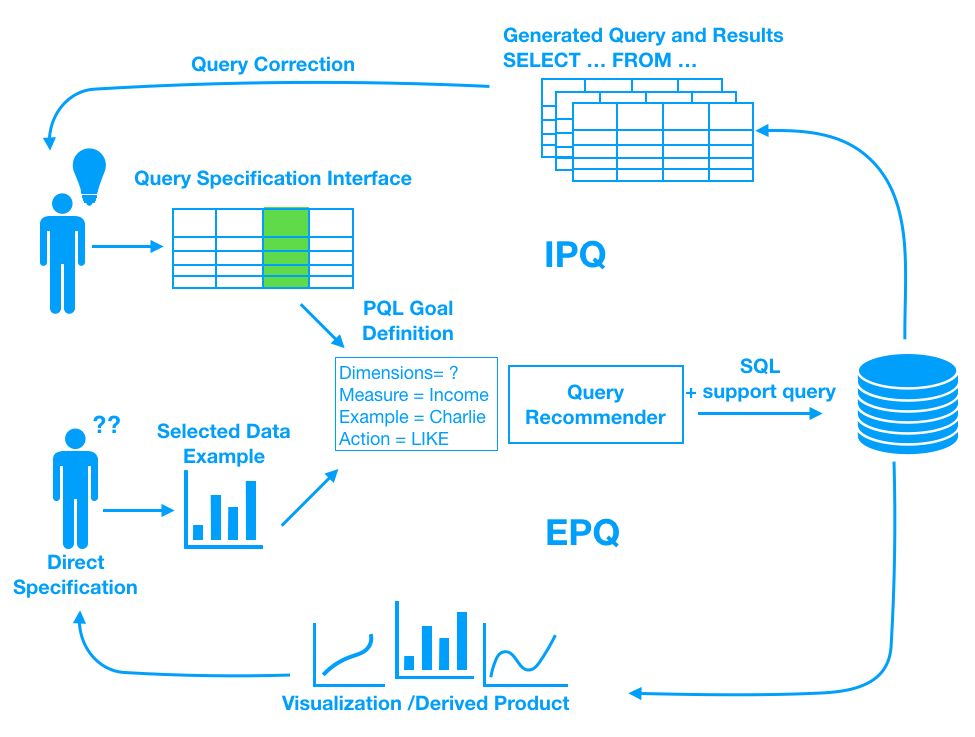
\includegraphics[width=\linewidth]{figures/system.png}
\caption{System architecture highlighting the relational and example partial query use cases. Example-based partial queries (EPQs) take in data examples based on what they have already seen and use this to jumpstart their query. Relational partial queries (RPQs) follow the conventional approach to querying a database where a user starts with a pre-existing idea of what he is looking for based on what he has already seen or know.  The users can move seamlessly across different query specification mechanisms to iteratively improve their query.}
\end{figure}
\section{Related Works}
\par Despite extensive work in database usability, there is an inevitable design trade-off between the query expressivity and interface usability\cite{Jagadish2007,Morton2014}. Here, we review three areas of related works in order of increasing usability: 
\subsection{General-Purposed Analytic Tools}

General-purposed analytic tools are systems that are designed for transforming, browsing, or visualizing data mainly via direct manipulation and specification. Manual specification is the conventional approach to querying a database where a user starts with a pre-existing idea of what she is looking for based on what she has already seen or know. However, formulating SQL queries that maps user's high-level intentions to specific query statements is challenging. Users often do not know what they want to query for without context. The extensibility of these systems or querying language also comes with the cost of potentially overloading the users with too many potential data actions to chose from. Recommendation and visual query building was developed to address these issues to help novices issue common queries, such as SPJ or basic aggregation.
\subsection{Data Recommendation}
Recommendation systems used for supporting analysts during exploratory analysis largely falls under three main categories: 1) Relational recommendations: what data slices, attributes, tables may be of interest to the user given prior history logs\cite{Khoussainova2010,Alborzi,Pal2017}, 2) Visualization recommendation: recommending interesting visualizations, intended to summarize and focus the user's attention onto particular portions of data\cite{Vartak2015,Wongsuphasawat2017}, and 3) Explanation recommendation: recommending possible explanations (queries that generated the results) from a given transformed tuple results (e.g. aggregation, top-k)\cite{Chapman2009,Wu2013,Roy2015}. Our proposed work is more similar to relational recommendation in spirit. However, 
these systems are often limited by the availability of a query workload to define a supervised metric of interestingness. For example, SnipSuggest addresses this problem by recommending relevant snippets of SQL queries based on partial queries (user's partially typed input) via auto-complete\cite{Khoussainova2010}. Likewise, \cite{Pal2017} make use of the assumption that an attribute is interesting if there is a derived table that make use of this attribute as constraint. Visual recommendation system such as Voyager make use of partial specification through ``wildcards'' to show appropriate visual encodings for all possible x,y based on the data type. While this works well for datasets with small number of attributes, since this approach does not rank visualizations, large numbers of plots will be generated when there are large numbers of attributes and would be difficult to interpret.
\subsection{Visual Query Builders}
Limited query type supported available + assumptions
\par Existing work in query-by-examples (QBE) asks users to provide I/O examples of the query to be synthesized\cite{Wang2017a,Wang2017}. However, if the user does not know what they are querying for, then they would not be able to come up with such an example. 
\par Visual query builders often consist of highly-usable interfaces that asks users for a specific set of information mapped onto a pre-defined query. Recent work in natural language querying have tried to address this by parsing adjectives and quantifiers and asking the users for additional information to resolve the ambiguity through form-based interface if needed. Similar to form-based or visual query builders\cite{Abouzied2012}, these systems are often based on templated queries with limited expressiveness in their linguistic and conceptual coverage, which makes it difficult for expert users to express complex queries. 
\cite{Jin2017}
\section{Motivation}
\par Given that there is no one size fit all interface for query specification for users of different expertise levels and workload, PQL is designed as a middle-layer between the interface and querying engine that can take in a wide spectrum of queries of different input types and degrees of specificity that could be potentially generated from different interfaces. As highlighted in Fig.\ref{system}, these can range from cold-start (no supervision) to input examples, input relations to complete specification.
%these two inter-related modes of data exploration, where data or bottom up approaches are initiated through data examples and framing comes from specifying distribution or relationships in a top-down manner.
\subsection{Application \#1: Spreadsheet Guidance}
\par A team of analyst is a given a dataset that consists of the reported income of individuals. They wanted to investigate whether there is any evidence of institutional bias on worker salaries. Given this large dataset with hundreds of attributes and records, they are unsure of where to start. The only thing they know is that they care about the Income column, so they specify this as the measure attribute of interest in PQL by brushing the Income column in yellow (Figure \ref{example} top). In this initial step, PQL tries to provide as much support information as it can by displaying a sample table of data records arranged in the order of increasing income, the attributes are displayed in the order of most to least importance, where importance is defined by how much the feature have an impact on the measure variable of interest. By convention, the primary key is always in the first column. These attribute-importance ranking techniques populates the most important relations that the users has to see in the first few visible columns.
\par Given this information, analyst A was still not able to infer anything about any particular column to ask a new question, but notices that Charlie has an incredibly low income compared to average. Using PQL specification interface, he uses the green paintbrush to highlight the record for Charlie and specifies the action to look for other records similar to Charlie. He notices that all of the returned records are all young children who work part-time jobs.
\begin{figure}[ht!]\label{example}
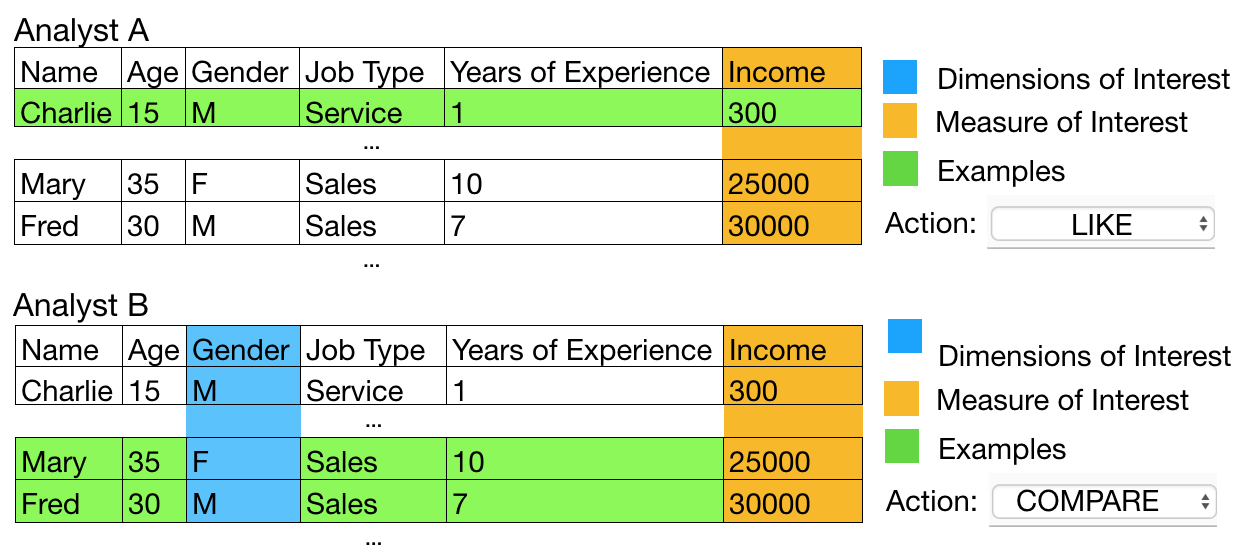
\includegraphics[width=\linewidth]{figures/example2.png}
\caption{One example of a potential interface that could be used for submitting PQL queries. Users can select examples or columns of interest. }
\end{figure}
\par Analyst B skims through the records and notices that despite Mary having more years of working experience than Fred, she is getting paid \$5000 less than him. He wants to find out whether employers are marginalizing the pay of certain individuals based on gender for the same job done. He colors the Gender column in yellow and the record of Mary and Fred in green, then specifies the ``COMPARE'' action (Figure \ref{example} bottom). Given this PQL specification consisting of a mix of records, dimensions and measure attributes, the example finding algorithm in PQL finds records that are similar to Fred AND Mary, while distinguishing these groups of records by gender. The results consist of two tables corresponding to males and females with similar credentials as Fred and Mary. Using the records and supporting overview statistics and histograms for the corresponding result-sets, analyst B finds that Gender is not a factor in determining Income and that the observed example was an anomaly and seeks for additional hypothesis that explains the difference between Mary and Fred.
%Given this hypothesis, he specifies a PQL query to find women who are in Sales and have similar years of experience as Mary and Fred. The PQL engine generates two support queries on this selected population to display the overview statistics and histograms of the selected subpopulation and its counterpart (i.e. men who are in Sales with similar years of experience).
\subsection{Application \#2: NLP Data Exploration}
There has been recent interest in NLP for data exploration systems that facilitates a more natural conversational approach version of business reporting for decision makers who may not have the expertise to formulate or time to explore the data comprehensively to gain quick insights\cite{tableauBIreport2018}. However, ambiguity is inherent to natural language queries\cite{Gao2015,Hoque2017}. Given that PQL can tolerate ambiguity and partial specification, it can directly execute the ambiguous query formulations.
\section{Formative Study}
\par In order to motivate the language design of PQL, we were interested in the space of queries that users would be interested in and the portion of data that they want use to achieve their analysis goals. We asked participants to browse through a real-world dataset that contains information about the home-rental site Airbnb's rental listings\footnote{\url{https://goo.gl/EUMQy6}}, consisting of 100088 rows and 16 columns. Participants were provided the study instructions, four example scenarios, and questionnaire via a Google Form\footnote{\url{https://goo.gl/forms/Y3lvxQsst3VIvoBs1}}. We ask participants to describe three envisioned scenarios of how people might analyze the given dataset. For each envisioned scenario, participants are required to describe the analysis goals and the analysis task for accomplishing the goal. Optionally, participants are also asked to specify whether there are any columns, rows/examples and other values of interest for the analysis. 
\par We have collected 27 example scenarios from 9 participants with prior experience with working with data. We performed a thematic analysis on the textual descriptions of the scenario task and objectives to obtain the results discussed in this section. The key features of interest such as task categorization and abstracted actions/goals were extracted from the anonymized raw responses\footnote{\url{https://goo.gl/GNtR7y}}.
\section{Discussion}
%Reflecting the two ---, PQL supports these two corresponding types of queries:  
Given the results from the formative study and existing systems in this space, we discuss a set of desiderata to motivate the language design of PQL, in order of most to least importance.
\subsection{Tolerant to ambiguity} 
PQL requires a model of inference that can make inference with incomplete specification, since 1) partial queries can be used for jump-starting the exploration of under-developed hypothesis and 2) queries can be iteratively refined and corrected as user gain more information about the data to update the model. 
\subsection{Workload-independent model} Model does not depend on a domain-specific query workload: Many existing systems makes use of information from query logs to provide ``typical workload'' query recommendations\cite{Morton2014,Kamat2016,Khoussainova2010}. However, the existence of such workloads is not commonly available outside of large enterprises or scientific collaboration setting. In addition, while PQL can be used for all stages of analysis, it is most beneficial to the users at the early-stages of data analysis. So if there is a pre-existing queries performed, it means that a detailed analysis had already been performed and the insights from that analysis (e.g. through documentations) should have given the analyst a better idea on what questions to ask next. Without the query workload, the model of inference must work with minimal user input and be updatable upon additional user input.
\subsection{Composability} PQL operators must be composable to increase the expressiveness of PQL in supporting a large class of ad-hoc queries, so that analysts are not constrained when exploring the types of questions they might want to ask.
\subsubsection{How common are the use of columns/rows of interest as query inputs?} 


\subsection{Supporting both records and relations as inputs} Given the prior work of how analyst make sense of their data\cite{Pirolli2005,Klein2006}, PQL must support both bottom-up example records and top-down relational specification of queries. As shown in the usage scenario, given the same data output, different analysts may have different interpretation and approach the same dataset and problem. %PQL enables analysts to seamlessly switch between the two modes of inquiry as shown in Figure \ref{architecture}.  %Popular theories in data sensemaking have suggested two different symbiotic modes of operations for understanding data. Pirolli and Card’s notional model describes information processing as an ``opportunistic mix'' between top-down (from theory to data) and bottom-up (from data to theory) tasks\cite{Pirolli2005}. Similarly, the Data/Frame theory suggests that the data analysis process is a closed-loop transition between an effort to recognize or construct a frame through data or defining connections amongst the seen data\cite{Klein2006}. 
	%\item Ability to suggest possible actions: The suggestion can come in two forms: 1) Given a partial query, suggest the possible queries that are \textit{simmilar in functionality} or 2) Given a data example or resultset, suggest possible next steps or actions that reflect \textit{simmilar data relationships}.
	%\item Model takes in feedback
	% \item Ability to generate explainations: Simmilarly explaination could be 1) by-example: data/record-level locality, or 2) by theory: membership or behaviour locality.
\subsection{Task Categorization and Discussion}
Fig. \ref{tasks} show the occurrences of tasks decomposed from the participants description. The focus of this discussion is on advanced multi-step tasks that emerged as a common pattern in study scenarios and its implications on the PQL language design.
\begin{figure}[ht!]\label{tasks}
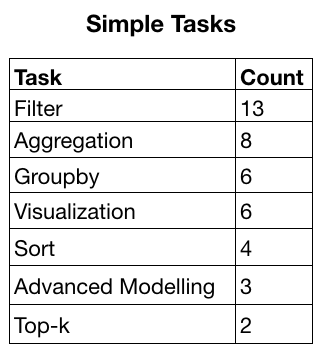
\includegraphics[width=0.5\linewidth]{figures/supported_tasks.png}
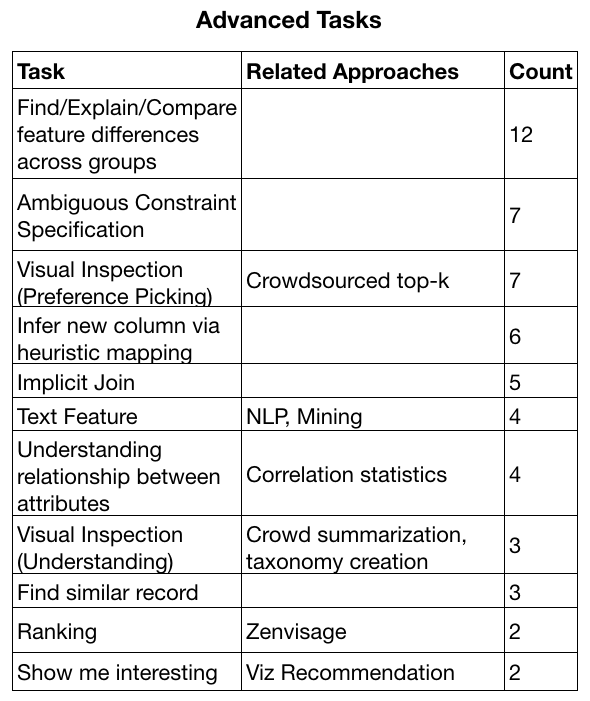
\includegraphics[width=0.5\linewidth]{figures/advanced_tasks.png}
\caption{Left: Tasks that can be represented as simple one-step queries. The common usage of these operators in a variety of scenarios explains their ubiquity in 
SQL, visual analytics, and other tools. Right: Advanced query operations that require a composition of operators or are not found in existing systems. }
\end{figure}
\\ \textbf{Find/Explain/Compare feature differences across groups:}
Comparisons across groups are one of the most common tasks for this dataset. Comparison is a multi-step process often involving: 1) Creation of groups, 2) creation of a corresponding ``others'' group to compare against, and 3) compare/computing statistics across created groups. Step one and two were done via filters, group-bys, or manual selection of tuples in the set. The third step often involves some type of aggregation over the created groups such as computing averages or correlation among groups and visualizing the results. D2, H2 also showcased examples of how analysts seeks explanations and features of what could distinguish one subgroup from another. 
\\ PQL can be designed to support both part of the group comparison task. First, PQL can better support manual creation of tuples selection sets by 1) making the group explicit, 2) summarization of selected tuples, and 3) suggesting similar tuples to add to the group. Similar to the idea in Data Tweening \cite{Khan2017}, group creation is a intermediary step that is in many cases not explicitly shown to the user. Even when group creation was performed through a top-down approach, we want to make the groups explicit by showing summaries or previews of the tuples in the group and ``others''. Suggestions 2 and 3 deals with the cases where group creation is done through manual selection of tuples. Summarization of selected tuples enables users to translate their bottom-up tuple inputs into top-down specification. For example, the users can chose several listings that seem appealing to them, the summarization of the selected group can inform them that all of their selected tuples satisfies a constraint. The users have the choice to either examine similar suggested tuples to add to the group or if they are confident that the proposed rule is captures what they are looking for, they can translate the tuple selection into a top-down formulation, which ensures that all tuples that satisfies this constraint are added to the created group. Similar formulation of mapping tuple examples to higher-level query specification have been proposed in DataPlay\cite{Abouzied2012} and other works on query synthesis via I/O examples\cite{Wang2017,Wang2017a}. However, we believe that with the more flexible preference and constraint model of filter specification (discussed in the next section) we will be able to make more realistic query filter recommendations.
\\ The comparison task itself can be ----- with two operators:
\begin{itemize}
\item DISTINGUISH $r_i$: Find the distinguishing feature of $r_i$.
\item COMPARE $\{r_1 ...r_n\}$: Compare why two or more records are different.
\end{itemize}
\\ \textbf{Ambiguous Constraint Specification:}
Another common trend we found in the way participants described the constraint was how ambiguous their specification of the constraints are. When considering this in terms of SQL WHERE clauses, these types of ambiguity can come in both sides of the inequality constraints. 
\\ First, what metrics or column should one use capturing the constraint of interest. This is often done through heuristic mapping, described in the next paragraph. Second, the user needs to figure out the cutoff criterion to set for defining inclusion/exclusion in the constrained group. For example, in scenario F1, 
\begin{quote}
John is a traveler looking for a house with free parking when spend his holiday in Orlando, if there's not a good match within certain limit, he would like to find one with payed parking lot.  
\end{quote}
the limit on what is defined as ``close'' is unspecified.  
\\ Amongst the 13 filter specification tasks, 4 proposed using sort to ease the process of visually inspecting the records to determine the filter criterion by eye. Another way that participants determined constraints was through visually filtering through similar entries. For example, scenario I1 describes a potential homeowner trying to determine ``how much money [he can]make per month given [his] current living/hosting situation''. He does this by ``filter[ing] out entries according to what's closest to my own hosting situation and look at rental prices.'' Additionally, an analyst can use the result of this manual filter to estimate the values of the desired criterion in the constraint.  For example, the analyst in scenario H1 ``wonders how much more expensive it would be to stay in a place that are cited as 'downtown' as opposed to those that do not. ''. He examines ``all rentals that have 'downtown' or similar in their description'' and checks ``if rentals [described] (sic) as 'downtown' are marked up'' by ``correlating it with their price and average rating/review''.
\\ Given the common visual filter-sort behavior in the earlier scenarios, we postulate that when filtering analysts distinguish between \textit{constraints} and \textit{preferences}. Constraints are strict inequalities found in SQL WHERE clauses that specifies membership of a tuple. Preferences are ``nice-to-haves'' that people want, but they do not necessary always need to be satisfied. In addition, preferences may not be strict inequalities, but general specifications such as ``the cheaper, nicer, safer the better''(A3, I2) or ``would be nice to have parking''(F1). In total, we found 6 scenarios in the form of `` finding `best' or top-k record while satisfying multiple constraints and preferences''. One potential direction for PQL is adding querying functionalities for specifying preference queries that can be used in conjunction with regular constraint clauses. 
\textbf{Visual Inspection}
The role of visual inspection of data records is often understated in exploratory analysis and in some situations can not be replaced by summarized insights (visualization or aggregate statistics). Visual inspection helps user gain an overview of the data and makes the underlying inference model more transparent to the users. This is important because in order for users to make corrections to the query, the users need to be able to trust and interpret the query results and understand why a particular query was suggested and executed. Several of the scenarios from the study have motivated the idea of using intuition gained from visually inspecting a carefully selected subset of the data (which can be results of a query) to facilitate ambiguity resolution. 
\\ One way to incorporate visual inspection is requesting the summarized insights from user after they performed visual inspections as feedback to help with the next iteration of query recommendation. For example, as an extension to preference picking, we may also consider how data types of an attribute impacts whether a user would be interested in a constraint or a preference. In the filter-sort scenarios, we find that people are more interested in first performing constraint filtering on quantitative attributes and then preference picking via visual inspection on text attribute columns, involving reading through listing names or reviews to make the top-k decision. In this case, the human analyst will be performing the visual top-k preference picking and returning these results to the system to continue the next step of the analysis.
\textbf{Infer new column via heuristic mapping}
Implicit Join
\textbf{Text Feature Discovery}
Existing text mining ----- importance, ---- will not be a core contribution of PQL 
\\ \textbf{Visual Inspection (Understanding)} (A1,D2,I2)
\\ \textbf{Find similar record}
\\ \textbf{Attribute relationship/ influence}
\\ \textbf{Ranking}
\\ \textbf{Show me interesting (Explore)}
Only 2 out of the 27 scenarios had examples where the participants did not specify concrete analysis task to support their goals. While this may be an artifact of choosing a highly-familiar dataset for the study, this result still invalidates our initial motivation for this work based on the notion that users often do not have a good idea on what they want to do when they first examine the data. Instead, we find that users generally have a reasonable high-level idea on what they want to do and the challenge is to support them in finding out how to do what they want to do. Since many proposed actions are half-baked or exploratory in nature, PQL's main goal should be to make it easier to test exploratory hypothesis and actions, even if such queries are ambiguous or underspecified, to minimize the barrier it takes to go from high-level ideas to actually testing them out.
\subsection{Preliminary ideas on Language Design and Problem Formulation}
PQL can be written in terms of action-operators and goal definitions. Goal definitions specifies the attributes and records that users are interested in. There are three types of goal definitions supported by PQL: 
\begin{itemize}
	\item Attribute-value of interest (e.g. GENDER= 'Female')
	\item Attribute of interest (e.g. GENDER=?): can either be a measure or dimension. Measure of interest have a special significance in the algorithm.
	%OBJECTIVE $M$ : Defining the measure value of interest during the analysis as M.
	\item Non-aggregated example records $\{r_1 ...r_n\}$: Point queries where all attribute-values are completely specified (e.g. Mary: GENDER=F, Age=35, ..., Income = 25k)
\end{itemize}
\begin{figure}[ht!]\label{nodeType}
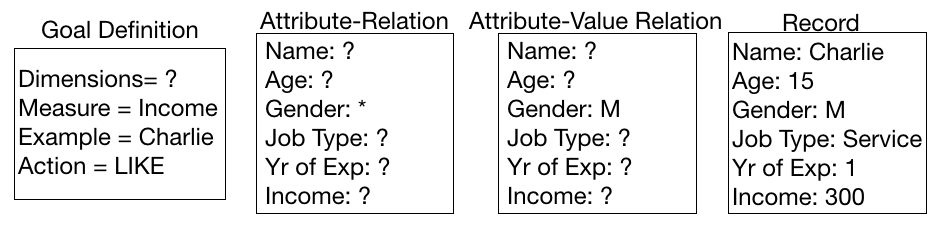
\includegraphics[width=\linewidth]{figures/nodeTypes.png}
\caption{An example PQL specification is shown on the left with ? denoting the underspecified values. The three types of goal definitions are shown in the right.}
\end{figure}
Any unspecified goal definitions is denoted with the special value ``?''. Action-operators can take a record ($r_i$) or relation ($A_i$) as inputs and outputs and performs some action. Action-operators can be decomposed as a set of goal definitions. Examples of action-operators includes:   
\begin{itemize}
  %\item DISTINGUISH $r_i$: Find the distinguishing feature of $r_i$.
	\item EXPLORE $\{A_1 ...A_n\}$: Overview or Drill-down to attribute(s) of interest.
	\item EXPLAIN $r_i$: Tracing the lineage of $r_i$.
	\item LIKE $\{r_1 ...r_n\}$: Find records that are similar to $r_i$.
	%\item COMPARE $\{r_1 ...r_n\}$: Compare why two or more records are different.
\end{itemize}
System detect sources of ambiguity through matching. Ambiguity resolution operators. 

\section{Problem Formulation}
Described below are two approaches that I am currently exploring for the problem of query recommendation given a PQL specification.
\subsection{Recommending the most important relations/examples for specified actions}
\par Given a limited space of operators, determining the best action to perform for a given input is not a hard problem, as the options could be simply recommended by matching desired inputs and selected by the user. In this case, the problem becomes a recommendation problem that involves finding the most suitable set of attributes or relations to perform the action-operator on.
\par We define relations and examples as nodes in a graph. As described earlier, examples are simply a special instance of relations where the values for all possible attributes are specified. Edges between the relations and examples can exist if the example contains the relation. Intuitively, a relation is ``important'' if many of the user's selected examples point to it. Conversely, an example is ``important'' if is pointed by many selected or high-influencing relations (i.e. measure attribute of interest strongly depends on the feature). Variants to PageRank-like algorithms such as HIT\cite{Kleinberg1999} may be suitable for this application in finding the most important node to recommend in a query. Solving this problem is challenging since the number of potential combination of attribute-value combination can be large for datasets with high-cardinality attributes or large numbers of attributes. In addition, how to find the appropriate ranges or bins to create attribute-value combinations for a numerical attribute (such as Age) is unclear.
\subsection{User Feedback for iterative steering in data-action space}
One alternative problem formulation is to incorporate user feedback to alleviate the problem of lack of user input. 
User feedback provides a way to collect additional inputs, since it is often easier for a user to make selections or ratings based on seen results, rather than coming up with query specification from scratch. While feedback has been prevalent in databases for the purpose of information retrieval(IR), the concept has not been explored extensively in interactive data exploration system. Most systems have focused on system-level feedback to aid the users in data exploration \cite{Nandi2013,Jiang2015}. However, the human action cycle of interaction requires closed feedback loop between user and the system\cite{Norman2013}. DataPlay provide a query correction tool for users to mark `want out', `keep in' examples to improve the query \cite{Abouzied2012}. Coming up with a right model for feedback is challenging since users often regard database queries to provide ``ground truth''(rather than varying degrees of relevance as in the case of IR), so the feedback information provided by the users will not be as simple as relevant/irrelevant, which makes inference harder.
\par Feedback also provides a mechanism in which we can collect more information about the user's intent to infer the missing fields in partial query. If we consider query recommendation as a search problem through the space of data and actions, a mixed-initiative interface that enables users to provide feedback as well as update their partial queries can help steer the recommended queries to reach the right balance between the multiple objectives (such as diversity, representative, interestingness, etc.). Contrary to the previous problem formulation, the interactive multi-objective optimization works on top of both the data-action space and seeks the most suitable query to perform on recommended relation/examples, rather than simply a search for the most important relation/examples to perform on a fixed query.
\section{Limitations}
The occurrences of the tasks discussed may simply be an artifact of the dataset chosen for this study. 
\section{Future Work}
For the course project, I surveyed related works, provided concrete examples from real-world datasets, and conducted a formative study to motivate the design choices of the PQL language to serve as a proof-of-concept to the potential applicability of PQL. The next steps of this project includes: 
\begin{enumerate}
\item Designing a complete set of functions, operators, and rules for the PQL language that fits the desiderata. (Desiderata \# 1, --)
\item Designing a model for feedback to enable query modification and correction, along with recommendation. (Desiderata \# 1, --)
\item Problem formulation that enables the query execution under (Desiderata \# 1, --)
Ensure that model of inference is easily interpretable by the users.
\item 
\end{enumerate}
I plan to distill these into a set of functions, operators and ---- supported by SQL and come up with a problem formulation that ----- making inference with partial or ambiguous specification and feedback based on these desiderata.
The project will focus on developing the problem formulation and potential algorithms for solving the query recommendation problem for PQL, as well as expanding on the details of the PQL language design. While I do not plan to build the system prototype.

Questions: 
- Given that in the user study, you found diverse set of use cases and tasks. How can PQL unify them all? 
- How does the common tasks found from the study different from existing systems like Zenvisage?
\bibliographystyle{abbrv}
\bibliography{reference}  
\end{document}
